\documentclass[12pt]{article}
\usepackage{amsmath}
\usepackage{amssymb}
\usepackage{amsfonts}
\usepackage{array}
\usepackage{graphicx}
\usepackage{mathrsfs}
\usepackage{multirow}
\usepackage{siunitx}
\usepackage{booktabs}
\usepackage{enumitem}
\usepackage[left=0.8in, right=0.8in, top=1in, bottom=1in]{geometry}
\usepackage{changepage}
\usepackage{longtable}

\bibliographystyle{IEEEtran}
% \setlength\topmargin{-1.1in} \addtolength\textheight{2.1in}
% \addtolength{\oddsidemargin}{-0.2in}
% \addtolength{\evensidemargin}{-0.1in} \textwidth 5.8in
\newcounter{questioncounter}
\newcounter{equestioncounter}
\setlength\parskip{10pt} \setlength\parindent{2em}

\begin{document}

\begin{titlepage}
\centering
\vspace*{\stretch{0.2}}
{\LARGE\textbf{Gesture Based Turn Signaling System }}\\[1cm] 
{\large\textbf{ECE 445 Design Document Spring 2024}}\\[0.3cm]
\rule{\textwidth}{1pt}\\
\vspace*{\stretch{2}}
{\Large Sultan Alnuaimi, Edan Elazar and Kaylan Wang}\\[0.5cm] 
{\small \{saltana2, eelazar, kaylanw2\}@illinois.edu}\\[0.5cm] 
{\small Professor: Viktor Gruev}\\[0.5cm]
{\small TA: Sanjana Pingali}\\[1cm]

\vspace*{\stretch{2}}
\end{titlepage} 

\tableofcontents 
\newpage
\section{Introduction}
\subsection{Problem}
Cyclists, skateboarders, and scooter riders often face 
challenges in signaling their intentions to drivers,
especially in low-light conditions. According to the CDC, 
1,000 cyclists die and 130,000 are injured every year on 
the road in the United States \cite{CDC2024BicycleSafety}. 
These numbers don’t include other riders sharing the road on 
things like skateboards and scooters. There are many interventions 
in place to prevent these accidents, such as fluorescent or 
retro-reflective clothing, or active lighting on the bicycle 
(required by law in most states) \cite{CDC2024BicycleSafety}, 
but the traditional method of using hand signals is not always 
visible or practical, particularly at night or during adverse 
weather conditions. This lack of clear communication can lead 
to dangerous situations on the road, as other motorists may 
fail to recognize the cyclist's intended maneuvers, or if an 
accident occurs. 

\subsection{Solution}

To address this issue, we propose the development of a gesture 
recognition-based turn signaling system for cyclists and scooter 
riders. This system will utilize a combination of sensors, such 
as accelerometers and gyroscopes, integrated into a wearable 
like a jacket. Then we process the sensor data to identify 
specific arm gestures made by the rider and activate corresponding 
LED signals. For example, if the rider extends their arm straight 
to the left, the left turn signal is activated, or if the rider 
indicates a stop, then the brake light is activated, and so on. 
Additionally, the sensors will be able to detect when the rider 
has had an accident or a crash, and activate a hazard signal. 

We propose placing an IMU above (or below depending on how hard 
it is to differentiate between movements) the elbow on each arm 
of the wearable. The microprocessor will then receive and process 
the data from the IMU, determining what kind of movement has been 
made. Then, depending on the movement, it will output a specific 
signal to the LEDs to display on the back and arms of the wearable. 

\newpage
\subsection{Visual Aid}
\begin{figure}[ht]
    \centering
    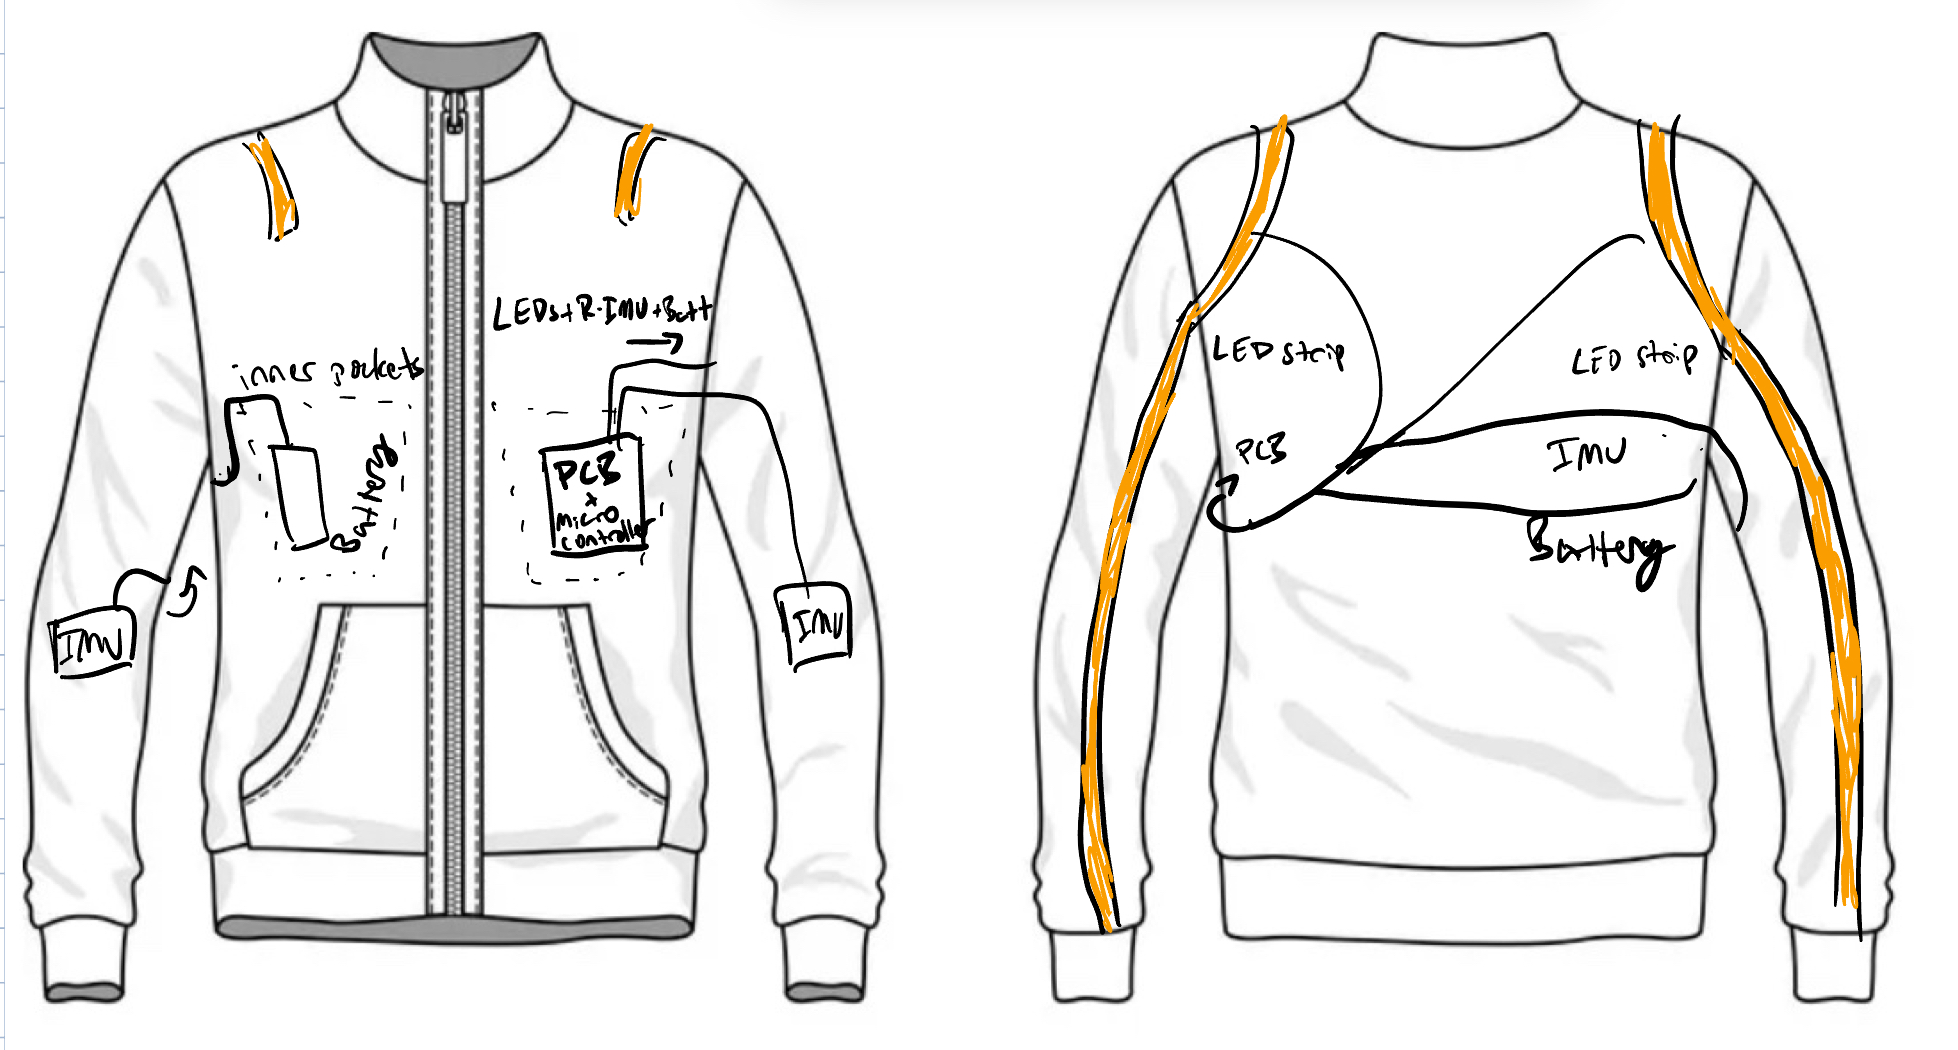
\includegraphics[width=0.8\textwidth]{visual_aid.jpg}
    \caption{Visual Aid mockup of the wearable \cite{VectorStock2024}}
    \label{fig:my_label}
\end{figure}
\subsection{High Level Requirements}
\begin{enumerate}
    \item The device should be able to correctly detect 
    predefined arm gestures (raising right/left arm for turn 
    signals, forearm down for slowing down) with a minimum accuracy of 90\%. 


    \item The device should be able to correctly map the arm 
    gestures into the different indications on the LEDs. The turn signal will be indicated by either the left or right side LED flashing orange, while the brake/slow down signal will be indicated by all LEDs turning red. A crash or accident will activate the hazard light, indicated by all LEDs flashing red. 

    \item The turn signals, brake lights, and hazard signals should all be visible and easily identifiable from a distance of at least 250 feet to ensure that they are clearly visible at both day and night. 


\end{enumerate}

\newpage
\section{Design}
\subsection{Block Diagram}
\begin{figure}[ht]
    \centering
    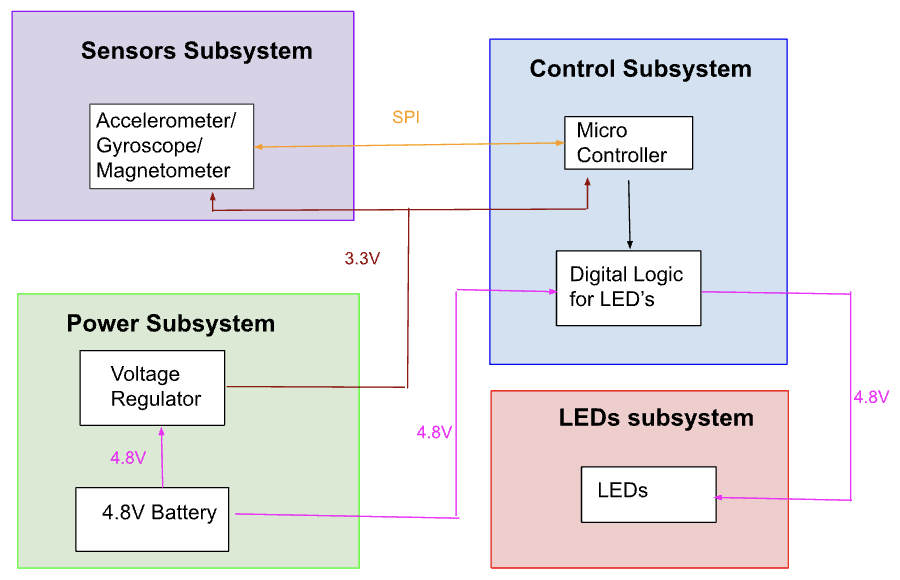
\includegraphics[width=0.8\textwidth]{block_diagram.png}
    \caption{Block Diagram of the system}
    \label{fig:my_label1}
\end{figure}

\subsection{Physical Design}
Tentative plan for physical design: For the LEDs, we can attach velcro strips at the wrist, elbow, back shoulder, and upper chest areas (both left and right sides), and attach the LED strip along the velcro strips. For the IMUs, place them into small drawstring bags and attach velcro to the outside of the bag and to the inner part of the jacket sleeve near the wrists. The velcro will allow for easier removability for the electronics to aid in debugging as well as for the user to be able to wash the jacket. The PCB and battery can be placed in the inner jacket pockets. For the wiring, we will be physically wiring the LEDs and IMU to the PCB through the inner part of the jacket, making a hole in the front upper chest area to route the LED wires from the outside to the inside to where the PCB will be placed. 
\subsection{Subsystem Requirements and Verifications}
    \subsubsection{Control Unit} 
    The control unit to be able to receive data through the SPI protocol from the sensors and analyze the data in order to route the 4.8V from the battery to power the LEDs. The data will consist of acceleration, rotational, and magnetic orientation data from the 9 degrees of freedom (9DoF) IMU. The PCB will contain the microcontroller, power the sensor suite, and contain digital logic to control the LEDs. We will use the 
    ESP32 microcontroller \cite{EspressifESP32} to process the data from the sensors 
    and output the correct signals to the LEDs. To turn the LEDs on and off via software, we will add transistors \cite{MicrochipVN10K} to the PCB, so that the microcontroller can control the power to the LEDs. The control unit will also use software (to be determined and tested) to filter the noise. This data will then be analyzed by the ESP32 to identify the gesture made by the user. This information will then be used to control the LED subsystem.
    \begin{table}[h]
        \centering
        \caption{Control Unit Subsystem Requirements and Verification}
        \begin{tabular}{p{0.45\linewidth}p{0.45\linewidth}}
        \toprule
        \textbf{Requirements} & \textbf{Verification} \\
        \midrule
        \begin{itemize}[leftmargin=*, nosep, after=\strut]
            \item Must be able to communicate with the sensors and LEDs through the PCB
            \begin{itemize}[nosep]
                \item Must be able to output 4.8±0.3V to the LEDs
                \item The accelerometer must be able to detect acceleration within ±1m/s.
                \item The magnetometer must be able to detect North.
                \item The gyroscope must be able to detect angular rate within ±15 dps.
            \end{itemize}
            \item Must be able to determine the correct turn signal from the IMU
            \item Must be able to turn on the LEDs based on the corresponding turn signal
            \begin{itemize}[nosep]
                \item Turn left: Must be able to flicker the left LED
                \item Turn right: Must be able to flicker the right LED
                \item Slow down: Must be able to turn on both LEDs
                \item Hazard: Must be able to flicker both LEDs
            \end{itemize}
        \end{itemize} &
        \begin{itemize}[leftmargin=*, nosep, after=\strut]
            \item Connect the IMU to the ESP such that the ESP can print the IMU acceleration readings from the accelerometer. Drop 3 times (once for each x, y, z axis), and verify that the acceleration is g±5m/s
            \item Connect the IMU to the ESP such that the ESP can print the IMU gauss reading from the magnetometer. Point the IMU in different directions and verify that the gauss peaks when pointing North.
            \item Connect the IMU to the ESP such that the ESP can print the IMU angular rate readings from the gyroscope. Spin the IMU using a motor and verify that the angular rate readings match the dps of the motor ±20 dps.
            \item Move the IMU and print on the ESP the detected turn signal. The printed line should match the turn signal being made.
            \item Move the IMU and use a multimeter to verify that a 4.8±0.3V signal is being output to the LEDs
        \end{itemize} \\
        \bottomrule
        \end{tabular}
        \end{table}
    \newpage

    \subsubsection{Power Subsystem} 
	We will use a 4.8V rechargeable battery (Li-Ion or LiPo) to 
    power the components, 4.8V for the LEDs, and use a voltage 
    regulator \cite{TI2023} to power the microcontroller and sensors at 3.3V. 
    The Power subsystem should be able to output 4.8V through the control unit to power the LEDs, as well as output 3.3V to power the Control and Sensors subsystems. 
    \begin{table}[h]
        \centering
        \caption{Power Subsystem Requirements and Verification}
        \begin{tabular}{p{0.45\linewidth}p{0.45\linewidth}}
        \toprule
        \textbf{Requirements} & \textbf{Verification} \\
        \midrule
        \begin{itemize}[leftmargin=*, nosep, after=\strut]
            \item Must be able to supply 3.3±0.3V to the IMUs and the ESP32
            \item Must be able to supply 4.8±0.3V to the LEDs
            \item The temperature of the battery should stay below 50 C during operation
            
        \end{itemize} &
        \begin{itemize}[leftmargin=*, nosep, after=\strut]
            \item The power will be turned on and a multimeter will be used to verify that the voltage output by one of the voltage regulators is 3.3±0.3V
            \item The power will be turned on and a multimeter will be used to verify that the voltage output by the other voltage regulator is 4.8±0.3V
            \item Measure the temperature using a thermometer during operation and ensure it is below 50 C
        \end{itemize} \\
        \bottomrule
        \end{tabular}
        \end{table}


    \subsubsection{Sensor Subsystem} 
    For the sensors, we will use a 3.3V 9dof IMU (accelerometer, 
    gyroscope, magnetometer) \cite{STMicroelectronics2015LSM9DS1} for each arm, and use the combined 
    data from both to determine the nature of the motion. In an 
    accident for example, the acceleration will spike, indicating 
    an accident. To distinguish between the other signals, we will
    use the gyroscope to determine the angle of the gesture. The 
    IMUs will be powered directly by the power subsystem through 
    a voltage regulator to step the voltage down to 3.3V. The 
    sensors will communicate with the ESP32 microcontroller 
    through SPI for data transfer. 
    The sensor subsystem should contain an IMU (accelerometer, gyroscope, and magnetometer) for each arm, read and controlled by the ESP32 microcontroller via an SPI signal. The data should contain acceleration, rotational, and cardinal direction data and should be filtered properly so as to not miss vital information and not cause false signals. The IMUs will be powered by a 3.3V input via the Power Subsystem.

    \begin{table}[h]
        \centering
        \caption{Sensor Subsystem Requirements and Verification}
        \begin{tabular}{p{0.45\linewidth}p{0.45\linewidth}}
        \toprule
        \textbf{Requirements} & \textbf{Verification} \\
        \midrule
        \begin{itemize}[leftmargin=*, nosep, after=\strut]
            \item The accelerometer must be able to detect acceleration within ±1m/s.
            \item The magnetometer must be able to detect North.
            \item The gyroscope must be able to detect angular rate within ±15 dps.
            
            
        \end{itemize} &
        \begin{itemize}[leftmargin=*, nosep, after=\strut]
            \item Connect the IMU to the ESP such that the esp can print the IMU acceleration readings from the accelerometer. Drop 3 times (once for each x, y, z, axis), and verify that the acceleration is g±5m/s
            \item Connect the IMU to the ESP such that the ESP can print the IMU gauss reading from the magnetometer. Point the IMU in different directions and verify that the gauss peaks when pointing North.
            \item Connect the IMU to the ESP such that the ESP can print the IMU angular rate readings from the gyroscope. Spin the IMU using a motor and verify that the angular rate readings match the dps of the motor ±20 dps.
            
        \end{itemize} \\
        \bottomrule
        \end{tabular}
        \end{table}
        \newpage
    \subsubsection{LED Subsystem} 
    The LED subsystem should be able to turn on the LEDs when powered by a 4.8V input from the control/power subsystems. We will use 2 LED strips with a length of 80 cm each. The strips will start from the upper chest toward the upper back, then it will go towards the wrist, refer to the visual aid for clarifications. 

    \begin{table}[h]
        \centering
        \caption{Sensor Subsystem Requirements and Verification}
        \begin{tabular}{p{0.45\linewidth}p{0.45\linewidth}}
        \toprule
        \textbf{Requirements} & \textbf{Verification} \\
        \midrule
        \begin{itemize}[leftmargin=*, nosep, after=\strut]
            \item Must be able to turn on and off given a 4.8V input.
            \item Must be bright enough for drivers to see from 250ft.
            
        \end{itemize} &
        \begin{itemize}[leftmargin=*, nosep, after=\strut]
            \item Connect the LEDs in series with a switch and 4.8V power source and verify that the LEDs turn on.
            \item Walk 250 ft away from the LEDs while they are on and check that they are visible
        
        \end{itemize} \\
        \bottomrule
        \end{tabular}
        \end{table}

\subsection{Tolerance Analysis}
We will be using several components operating at 3.3V and a 4.8V 
battery that allows recharging. Therefore we need to use a 
voltage regulator to step down the voltage for the sensors 
and the ESP32. Considering that our product is a wearable, it is important that the component, specifically the linear regulator, doesn't get too hot. We can calculate the change in temperature of the linear regulator by first calculating the power dissipated using $I_{\text{out}} (V_{\text{in}} - V_{\text{out}})$ and multiplying it by the thermal resistance of the linear regulator ($\Theta_{jc}$).

\noindent ESP32 worst case current draw: 355 mA

\noindent 2 IMUs, current draw for each: 4.6 mA

\noindent Total current draw: 364.2 mA

\noindent The assumed ambient temperature: 25°C 
\[
\Delta T = I_{\text{out}} (V_{\text{in}} - V_{\text{out}}) (\Theta_{\text{jc}}) = 0.36 \times (4.8 - 3.3) \times 5 = 2.7^\circ\text{C}
\]
\[
\text{Final Temperature} = \Delta T + \text{Ambient Temperature} = 27.7^\circ\text{C}
\]

\noindent The temperature rise is well within the operating range of the voltage regulator as well as not too warm for the user, so we can use it for our design.

\newpage
\section{Cost and Schedule}

\subsection{Cost}
The total cost of parts will be approximately $\$141.60$ and the expected labor costs are calculated as $\$40/hrs * 2.5 * 60 hrs = \$6,000$. This will be applied to all 3 team members so the total labor cost is $\$6,000 * 3 = \$18,000$. This comes out to a total cost of $\$18,141.60$.
\begin{figure}[ht]
    \centering
    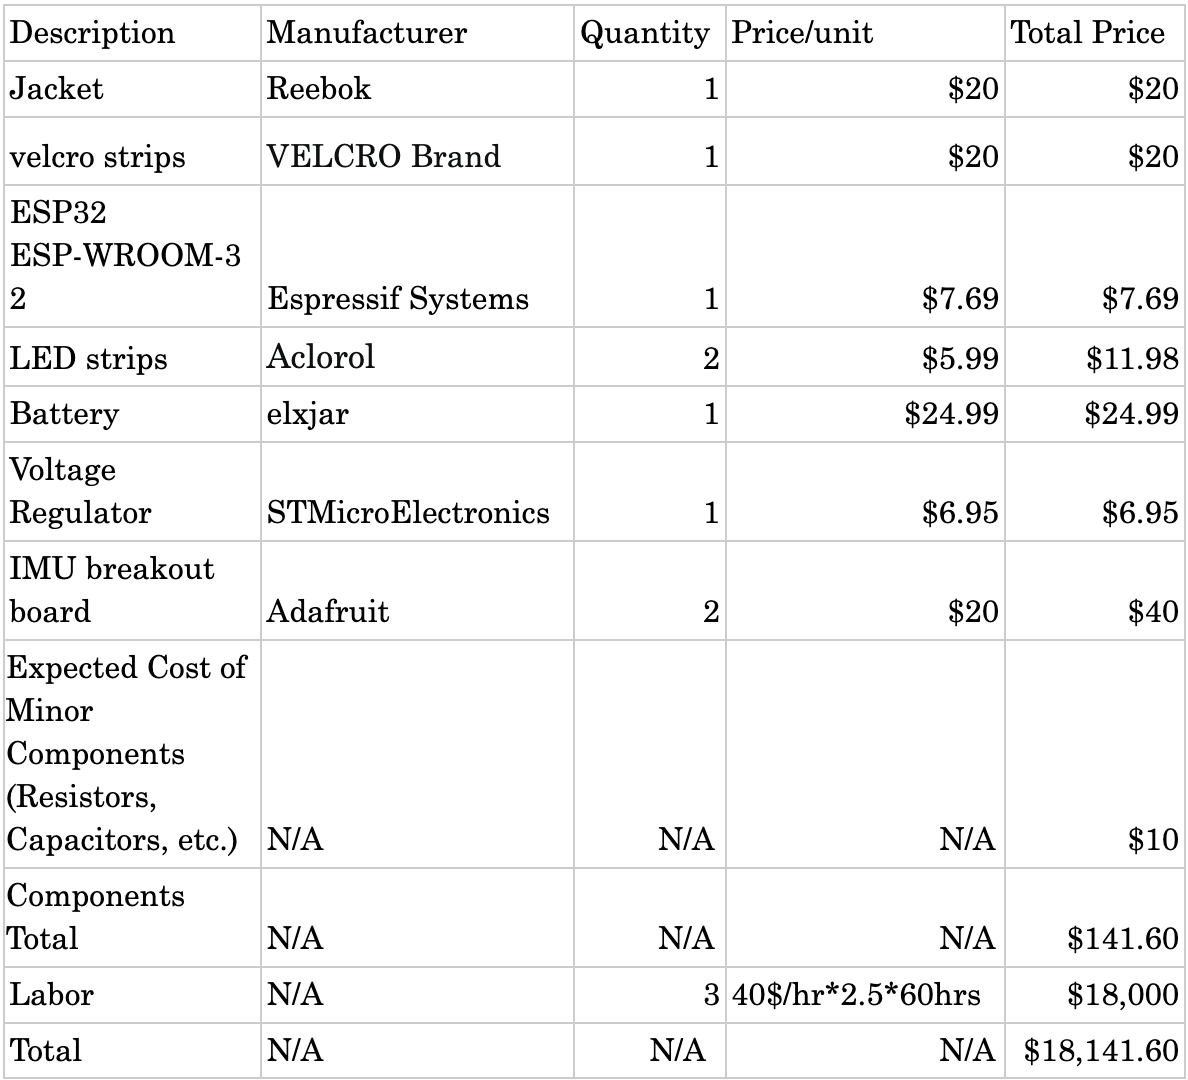
\includegraphics[width=1\textwidth]{cost_analysis.png}
    \caption{Cost Analysis}
    \label{fig:my_label2}
\end{figure}

\newpage
\subsection{Schedule}
\begin{figure}[ht]
    \centering
    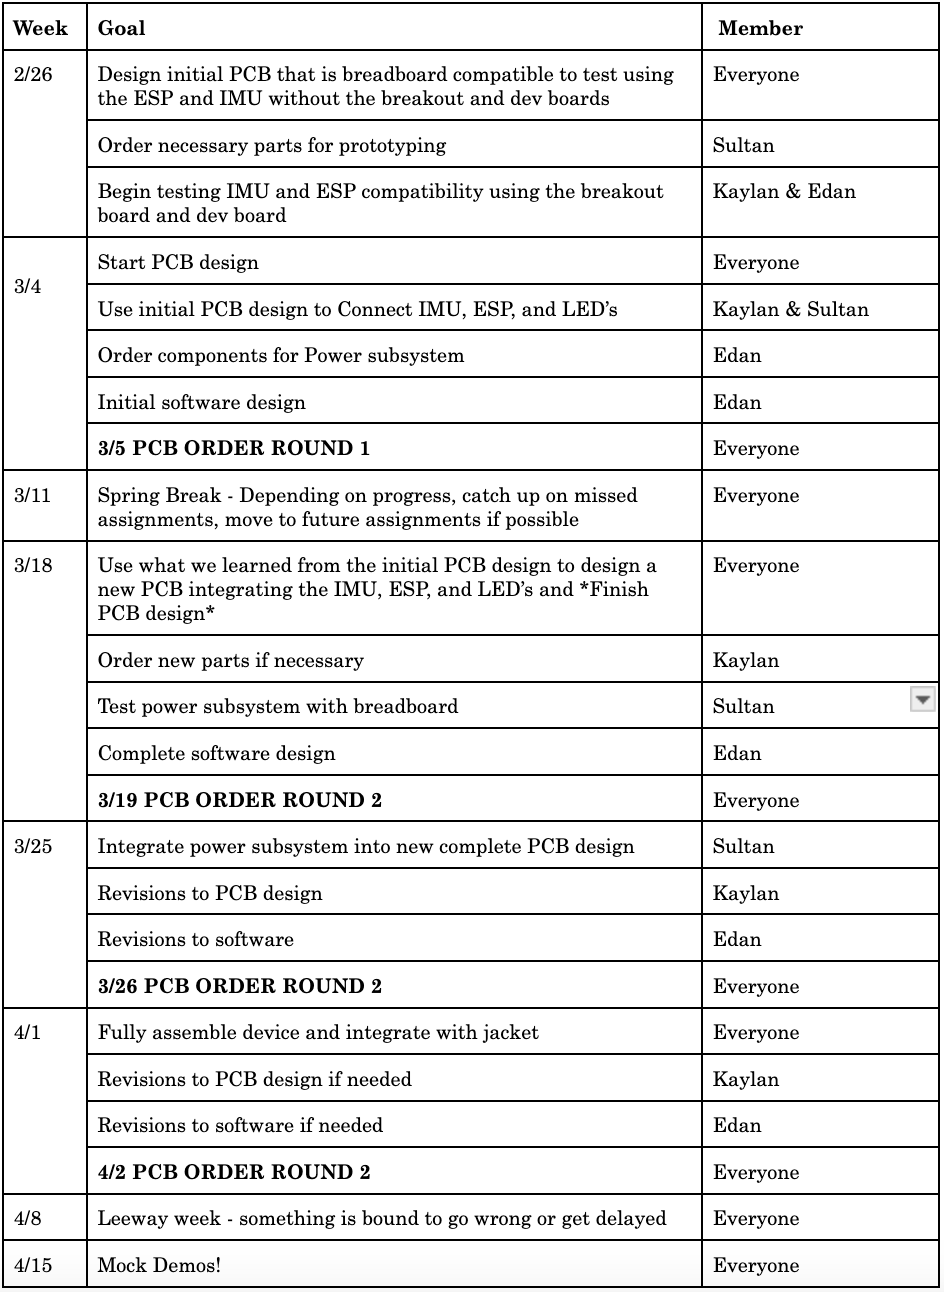
\includegraphics[width=0.70\textwidth]{schedule.png}
    \caption{Schedule of the project}
    \label{fig:my_label3}
\end{figure}
\section{Ethics and Safety}
\subsection{Ethical Considerations}
The biggest concern as it relates to ethics and safety for 
this project is with regard to the safety of the user and 
those on the road around the user. Under the IEEE code of 
ethics, we are required to prioritize the 
safety of the public \cite{IEEEethics2024}. If the wearable isn’t user
friendly enough, or restricts any movements, this can lead 
to potentially catastrophic accidents. We can solve this by 
integrating the electronics out of the way of the user, 
such as in the inner pockets of the jacket (for the PCB 
and battery), and providing ample slack in the wires 
throughout. This will allow the user to move more naturally.
Another concern might be the privacy of the user \cite{IEEEethics2024}
because we will be collecting and processing data constantly 
during a ride/commute. We can limit the data collection to 
IMU data, so that nothing personally identifiable is
collected, as well as deleting any data past a certain 
period of time. 




\subsection{Safety Considerations}
We have to consider the brightness of the LEDs, and if they can be distracting to other drivers and pedestrians. Having bright LEDs can be beneficial for low light or adverse conditions, but can also be harmful if they dazzle other drivers, impairing their vision. There aren’t any safety regulatory requirements for LEDs for bicycles relating to the brightness of the lights, so we make sure we are following the vehicle regulations for turn signals. \cite{CFR571_108} There are also consumer product safety standards that we need to follow for wearable technology, such as those related to electronics devices and battery safety. It is also important to note that wearing a battery is always dangerous. Because of this we will be following the guidelines on battery safety outlined by UIUC \cite{UIUCBatterySafety2023}. In addition, we verified in our tolerance analysis that the linear regulators will not get too hot to ensure the safety of the users.


\newpage
\bibliography{references}


\end{document} 